\documentclass[a4paper,12pt]{article}
\usepackage[slovene]{babel}
\usepackage[utf8]{inputenc}
\usepackage[T1]{fontenc}
\usepackage{lmodern}
\usepackage{amsmath, amsfonts, amsthm, amssymb}
\usepackage{a4wide}
\usepackage{listings}
\usepackage{xcolor}
\usepackage{graphicx}
\usepackage{float}
\usepackage[a4paper, margin=2.5cm]{geometry}
\usepackage{titlesec}
\usepackage{indentfirst}
\usepackage{dsfont}
\usepackage{tkz-graph}


% Nastavitev za prikaz kode
\lstset{
  basicstyle=\ttfamily,
  showspaces=false,                % Skrij presledke
  showstringspaces=false,          % Skrij presledke v nizih
  columns=fullflexible,            % Prilagodljivi presledki
  keepspaces=true,                 % Ohrani presledke
  xleftmargin=0.5cm,               % Dodatni levi rob za okvir
  xrightmargin=0.5cm,              % Dodatni desni rob za okvir
  breaklines=true,                % Brez prelamljanja vrstic
  aboveskip=10pt,                  % Razmik nad kodo
  belowskip=10pt,                  % Razmik pod kodo
  language=Python,                % Jezik kode
  keywordstyle=\color{blue},      % Barva ključnih besed
  stringstyle=\color{green!50!black}, % Barva nizov
  commentstyle=\color{gray},      % Barva komentarjev
  inputencoding=utf8,       % Podpora za UTF-8 kodiranje
}


\newtheorem{izrek}{Izrek}[section]

\theoremstyle{definition}
\newtheorem{definicija}{Definicija}[section]

\newtheorem{trditev}{Trditev}[section]

\theoremstyle{remark}
\newtheorem*{opomba}{Opomba}

\theoremstyle{definition}
\newtheorem*{primer}{Primer}


\begin{document}

\begin{titlepage}
    \begin{center}
        \vspace*{5cm}

        \Huge
        \textbf{Vozliščne, povezavne in mešane metrične dimenzije}

        \vspace{0.5cm}
        \LARGE
        Projekt za finančni praktikum

        \vspace{1.5cm}

        \textbf{Lucija Tekavc}

        \vfill

        \Large
        Fakulteta za matematiko in fiziko\\
        20. 12. 2024
    \end{center}
\end{titlepage}


\section*{Definicije}

\begin{definicija}\label{def1}
    Vozlišče $s \in V(G)$ \textsc{razreši} par vozlišč $v$ in $u \in V(G)$,
    če velja: $d(s, v) \neq d(s, u)$. \\
    \textsc{Razrešljiva množica (za vozlišča)} $S$ je množica, za katero velja, da je
    vsak par vozlišč iz $V(G)$ razrešen z nekim elementom iz S.
\end{definicija}

\begin{definicija}
    \textsc{(Vozliščna) metrična dimenzija} grafa $G$ je moč najmanjše
    razrešljive množice za vozlišča, označimo z $dim(G)$.
\end{definicija}

\begin{definicija}
    \textsc{Razdalja do povezave} je razdalja do bližlega vozlišča na tej
    povezavi, tj. $\forall s \in V(G). \forall e = uv \in E(G).d(s, e)=min\{d(s,u),d(s,v)\}$.
\end{definicija}

\begin{definicija}
    \ref{def1} razširimo še na povezave in mešane povezave in vozlišča, tj.
    $s \in V(G)$ \textsc{razreši} par $x, y \in \{V(G), E(G)\}$, če
    $d(s, x) \neq d(s, y)$.
\end{definicija}

\begin{definicija}
    \textsc\b{Povezavna metrična dimenzija} grafa $G$ je moč najmanjše
    razrešljive množice za povezave, označimo $edim(G)$.
\end{definicija}

\begin{definicija}
    \textsc\b{Mešana metrična dimenzija} grafa $G$ je moč najmanjše
    razrešljive množice za vozlišča, povezave in mešano, označimo $mdim(G)$.
\end{definicija}

\section*{Cilji projekta}

V okviru projekta sem imela nalogo, da:
\begin{itemize}
    \item napišem funkcije za določanje vseh treh metričnih dimenzij,
    \item poiščem grafe, za katere velja $dim(G)=edim(G)=mdim(G)$
    \item poiščem grafe, za katere velja $mdim(G)=dim(G)+edim(G)$
\end{itemize}

\newpage
\section*{Funkcije}

\subsection*{Pomožna funkcija za določanje razdalje do povezave}
\begin{lstlisting}
def get_edge_to_vertex_distances(G):
    M = G.adjacency_matrix()
    distances = G.distance_all_pairs()

    dist_to_edges = {}

    for i, j in itertools.combinations(range(M.nrows()), 2):
        if M[i][j] != 1:
            continue
        list_of_dist_to_uv = zip(
            distances[i].values(), distances[j].values()
        )
        dist_to_edges[(i,j)] = {
            index: min(tup)
            for index, tup in enumerate(list_of_dist_to_uv)
        }

    return dist_to_edges
\end{lstlisting}


\subsection*{Vozliščna metrična dimenzija}

\begin{lstlisting}
def get_metric_dimension(G):
    V = G.vertices()
    assert V == list(range(len(V)))

    lp = sg.MixedIntegerLinearProgram(maximization=False)
    x = lp.new_variable(binary=True)
    lp.set_objective(sum(x[v] for v in V))

    for u, v in itertools.combinations(V, 2):
        vertices = [
            w for w in V if G.distance(w, u) != G.distance(w, v)
        ]
        lp.add_constraint(sum(x[w] for w in vertices) >= 1)

    lp.solve()

    resolving_set = [v for v in V if lp.get_values(x[v]) == 1]
    metric_dimension = len(resolving_set)
    return metric_dimension
\end{lstlisting}

\newpage
\subsection*{Povezavna metrična dimenzija}

\begin{lstlisting}
def get_edge_metric_dimension(G, dist_to_edges):
    M = G.adjacency_matrix()
    E = G.edges(labels=False)
    V = G.vertices()

    lp = sg.MixedIntegerLinearProgram(maximization=False)
    x = lp.new_variable(binary=True)
    lp.set_objective(sum(x[v] for v in V))

    for e_ix, f_ix in itertools.combinations(range(len(E)), 2):
        dist_to_e = dist_to_edges[E[e_ix]]
        dist_to_f = dist_to_edges[E[f_ix]]
        vertices = [v for v in V if dist_to_e[v] != dist_to_f[v]]

        lp.add_constraint(sum(x[w] for w in vertices) >= 1)

    lp.solve()

    resolving_set = [v for v in V if lp.get_values(x[v]) == 1]
    edge_metric_dimension = len(resolving_set)
    return edge_metric_dimension
\end{lstlisting}

\subsection*{Mešana metrična dimenzija}

\begin{lstlisting}
def get_mixed_metric_dimension(G, dist_to_edges):
    M = G.adjacency_matrix()
    E = G.edges(labels=False)
    V = G.vertices()
    v_distances = G.distance_all_pairs()
    v_distances.update(dist_to_edges)

    lp = sg.MixedIntegerLinearProgram(maximization=False)
    x = lp.new_variable(binary=True)
    lp.set_objective(sum(x[v] for v in V))

    for (_, dist_to_i), (_, dist_to_j) in
        itertools.combinations(v_distances.items(), 2):
        vertices = [v for v in V if dist_to_i[v] != dist_to_j[v]]
        lp.add_constraint(sum(x[w] for w in vertices) >= 1)

    lp.solve()
    resolving_set = [v for v in V if lp.get_values(x[v]) == 1]
    mixed_metric_dimension = len(resolving_set)
    return mixed_metric_dimension
\end{lstlisting}

Vse funkcije za iskanje dimenzije delujejo na podlagi celoštevilskega
linearnega programa (pri čemer sta $y$ in $z$ lahko vozlišči, povezavi ali mešano
glede na dimenzijo):

$$ min(\sum_{s\in V(G)}x(s)) $$
$$ \text{p.p. }
    A_{(y, z), s} = \mathds{1}(d(y, s) \neq d(z, s)) $$
$$   x(s) = \mathds{1}(s \in S) $$
$$   A_{(y, z), s} \cdot x(s) \geq 1 $$

\section*{Iskanje grafov}

\begin{lstlisting}
for n in range(1, max_n + 1):

    for i, g in enumerate(sg.graphs.nauty_geng("{0} -c".format(n))):

        dim = get_metric_dimension(g)
        dist_to_edges = get_edge_to_vertex_distances(g)
        edim = get_edge_metric_dimension(g, dist_to_edges)
        mdim = get_mixed_metric_dimension(g, dist_to_edges)

        if dim == edim == mdim:
            g.export_to_file(f"file_name", format="gexf")
            correct_graphs_eq.append(g)
        elif mdim == dim + edim:
            g.export_to_file(f"file_name", format="gexf")
            correct_graphs_mdim.append(g)
\end{lstlisting}

To je rahlo preoblikovana koda, s katero sem iskala grafe. Iterirala sem čez
vse povezane grafe z $n$ vozlišči. Za vsakega sem zračunala vse dimenzije in
nato le preverila, ali pogoji veljajo.

\subsection*{Zahteve za delovanje funkcij}

Koda je napisana v Pythonu 3.12 s Sage 10.4, naloženim s conda okoljem.
Poleg tega je potrebno imeti operacijski sistem na podlagi Unix.

\subsection*{Časovna zahtevnost}

Program je zelo časovno zahteven, saj iterira čez vse povezane grafe na določenem
številu vozlišč. Na vsakem nato naredi kar 4 trojne \texttt{for} zanke, eno vedno
čez vsa vozlišča, dve pa čez vozlišča, povezave ali oboje.\\
\indent Zaradi tega (in da se koda ne ponavlja identično) sem ločila funkcijo za
računanje razdalj do povezav, saj v dokumentaciji za Sage nisem našla nobene
že vgrajene. Sicer bi se še enkrat po nepotrebnem računale stvari v zahtevnosti
$O(V^3)$. \\
\indent To vsebinsko sicer ni najboljše, saj je kot argument v funkciji
graf $G$, na katerega so razdalje vezane, torej bi se lahko zlorabilo funkciji
za povezavne in mešane dimenzije, če bi vstavili razdalje nepovezanega grafa.\\
\indent Pri izvajanju kode se je izkazalo, da je bilo realistično v tako malo časa (dveh dneh)
pregledati le vozlišča do 10, pri čemer je bilo za 10 pregledanih le 2 milijona
od 11.716.571.


\section*{Analiza}

\subsection{$dim(G) = edim(G) = mdim(G)$}
\vspace{0.5cm}

Najprej si oglejmo, če je kako povezano število vozlišč in
metrične dimenzije, ko so te med seboj enake.

\begin{figure}[H]
    \centering
    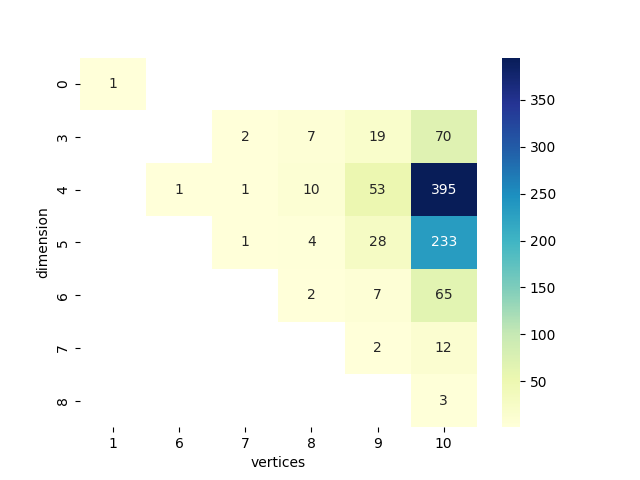
\includegraphics[width=0.9\textwidth]{eq_heatmap.png}
    \caption{Povezava med številom vozlišč in metrično dimenzijo pri $dim = edim = mdim$}
\end{figure}

\indent Za naše grafe odkrijemo, da zelo izstopa $dim(G) = 4$,
ki je pri kar štirih od 6 vozliščih najbolj zastopana podvojena
dimenzija. Na splošno se zdi trend, da so grafi dimenzije konkavni
z maksimumom v 4. \\
\indent Zaradi tega sem naredila KDE (Kernel Density Estimate)
graf, ki vsaj za majhno število vozlišč potrdi hipotezo, da se vozliščna,
povezavna in mešana dimenzija največkrat ujemajo, če se bližamo 4.

\begin{figure}[H]
    \centering
    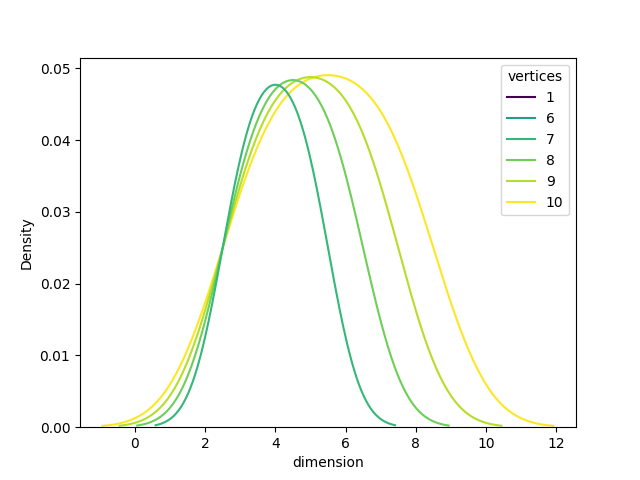
\includegraphics[width=0.8\textwidth]{eq_kdeplot.png}
    \caption{KDE graf po vozliščih za enake metrične dimenzije}
\end{figure}

\begin{figure}[H]
\centering

% 6_71_graph_d4
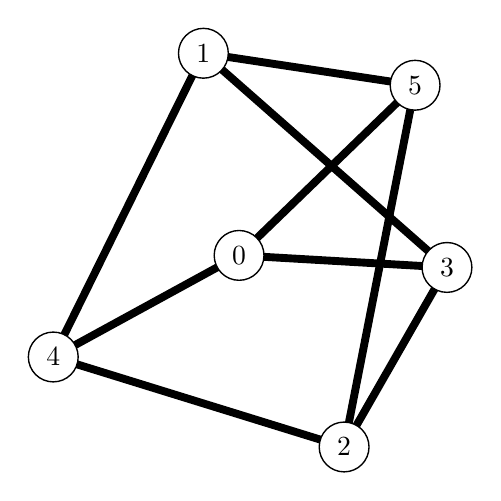
\begin{tikzpicture}
\definecolor{cv0}{rgb}{0.0,0.0,0.0}
\definecolor{cfv0}{rgb}{1.0,1.0,1.0}
\definecolor{clv0}{rgb}{0.0,0.0,0.0}
\definecolor{cv1}{rgb}{0.0,0.0,0.0}
\definecolor{cfv1}{rgb}{1.0,1.0,1.0}
\definecolor{clv1}{rgb}{0.0,0.0,0.0}
\definecolor{cv2}{rgb}{0.0,0.0,0.0}
\definecolor{cfv2}{rgb}{1.0,1.0,1.0}
\definecolor{clv2}{rgb}{0.0,0.0,0.0}
\definecolor{cv3}{rgb}{0.0,0.0,0.0}
\definecolor{cfv3}{rgb}{1.0,1.0,1.0}
\definecolor{clv3}{rgb}{0.0,0.0,0.0}
\definecolor{cv4}{rgb}{0.0,0.0,0.0}
\definecolor{cfv4}{rgb}{1.0,1.0,1.0}
\definecolor{clv4}{rgb}{0.0,0.0,0.0}
\definecolor{cv5}{rgb}{0.0,0.0,0.0}
\definecolor{cfv5}{rgb}{1.0,1.0,1.0}
\definecolor{clv5}{rgb}{0.0,0.0,0.0}
\definecolor{cv0v3}{rgb}{0.0,0.0,0.0}
\definecolor{cv0v4}{rgb}{0.0,0.0,0.0}
\definecolor{cv0v5}{rgb}{0.0,0.0,0.0}
\definecolor{cv1v3}{rgb}{0.0,0.0,0.0}
\definecolor{cv1v4}{rgb}{0.0,0.0,0.0}
\definecolor{cv1v5}{rgb}{0.0,0.0,0.0}
\definecolor{cv2v3}{rgb}{0.0,0.0,0.0}
\definecolor{cv2v4}{rgb}{0.0,0.0,0.0}
\definecolor{cv2v5}{rgb}{0.0,0.0,0.0}
%
\Vertex[style={minimum size=1.0cm,draw=cv0,fill=cfv0,text=clv0,shape=circle},LabelOut=false,L=\hbox{$0$},x=2.3599cm,y=2.433cm]{v0}
\Vertex[style={minimum size=1.0cm,draw=cv1,fill=cfv1,text=clv1,shape=circle},LabelOut=false,L=\hbox{$1$},x=1.9066cm,y=5.0cm]{v1}
\Vertex[style={minimum size=1.0cm,draw=cv2,fill=cfv2,text=clv2,shape=circle},LabelOut=false,L=\hbox{$2$},x=3.6937cm,y=0.0cm]{v2}
\Vertex[style={minimum size=1.0cm,draw=cv3,fill=cfv3,text=clv3,shape=circle},LabelOut=false,L=\hbox{$3$},x=5.0cm,y=2.28cm]{v3}
\Vertex[style={minimum size=1.0cm,draw=cv4,fill=cfv4,text=clv4,shape=circle},LabelOut=false,L=\hbox{$4$},x=0.0cm,y=1.1429cm]{v4}
\Vertex[style={minimum size=1.0cm,draw=cv5,fill=cfv5,text=clv5,shape=circle},LabelOut=false,L=\hbox{$5$},x=4.5952cm,y=4.5939cm]{v5}
%
\Edge[lw=0.1cm,style={color=cv0v3,},](v0)(v3)
\Edge[lw=0.1cm,style={color=cv0v4,},](v0)(v4)
\Edge[lw=0.1cm,style={color=cv0v5,},](v0)(v5)
\Edge[lw=0.1cm,style={color=cv1v3,},](v1)(v3)
\Edge[lw=0.1cm,style={color=cv1v4,},](v1)(v4)
\Edge[lw=0.1cm,style={color=cv1v5,},](v1)(v5)
\Edge[lw=0.1cm,style={color=cv2v3,},](v2)(v3)
\Edge[lw=0.1cm,style={color=cv2v4,},](v2)(v4)
\Edge[lw=0.1cm,style={color=cv2v5,},](v2)(v5)
%
\end{tikzpicture}
\caption{$dim(G) = edim(G) = mdim(G) = 4$}
\end{figure}


% 9_9941_graph_d3
\begin{figure}[H]
\centering
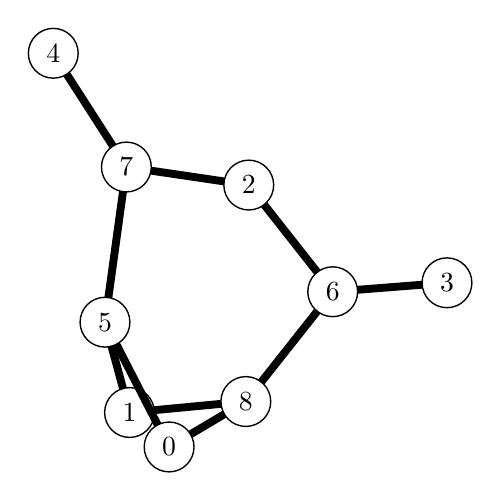
\begin{tikzpicture}
\definecolor{cv0}{rgb}{0.0,0.0,0.0}
\definecolor{cfv0}{rgb}{1.0,1.0,1.0}
\definecolor{clv0}{rgb}{0.0,0.0,0.0}
\definecolor{cv1}{rgb}{0.0,0.0,0.0}
\definecolor{cfv1}{rgb}{1.0,1.0,1.0}
\definecolor{clv1}{rgb}{0.0,0.0,0.0}
\definecolor{cv2}{rgb}{0.0,0.0,0.0}
\definecolor{cfv2}{rgb}{1.0,1.0,1.0}
\definecolor{clv2}{rgb}{0.0,0.0,0.0}
\definecolor{cv3}{rgb}{0.0,0.0,0.0}
\definecolor{cfv3}{rgb}{1.0,1.0,1.0}
\definecolor{clv3}{rgb}{0.0,0.0,0.0}
\definecolor{cv4}{rgb}{0.0,0.0,0.0}
\definecolor{cfv4}{rgb}{1.0,1.0,1.0}
\definecolor{clv4}{rgb}{0.0,0.0,0.0}
\definecolor{cv5}{rgb}{0.0,0.0,0.0}
\definecolor{cfv5}{rgb}{1.0,1.0,1.0}
\definecolor{clv5}{rgb}{0.0,0.0,0.0}
\definecolor{cv6}{rgb}{0.0,0.0,0.0}
\definecolor{cfv6}{rgb}{1.0,1.0,1.0}
\definecolor{clv6}{rgb}{0.0,0.0,0.0}
\definecolor{cv7}{rgb}{0.0,0.0,0.0}
\definecolor{cfv7}{rgb}{1.0,1.0,1.0}
\definecolor{clv7}{rgb}{0.0,0.0,0.0}
\definecolor{cv8}{rgb}{0.0,0.0,0.0}
\definecolor{cfv8}{rgb}{1.0,1.0,1.0}
\definecolor{clv8}{rgb}{0.0,0.0,0.0}
\definecolor{cv0v5}{rgb}{0.0,0.0,0.0}
\definecolor{cv0v8}{rgb}{0.0,0.0,0.0}
\definecolor{cv1v5}{rgb}{0.0,0.0,0.0}
\definecolor{cv1v8}{rgb}{0.0,0.0,0.0}
\definecolor{cv2v6}{rgb}{0.0,0.0,0.0}
\definecolor{cv2v7}{rgb}{0.0,0.0,0.0}
\definecolor{cv3v6}{rgb}{0.0,0.0,0.0}
\definecolor{cv4v7}{rgb}{0.0,0.0,0.0}
\definecolor{cv5v7}{rgb}{0.0,0.0,0.0}
\definecolor{cv6v8}{rgb}{0.0,0.0,0.0}
%
\Vertex[style={minimum size=1.0cm,draw=cv0,fill=cfv0,text=clv0,shape=circle},LabelOut=false,L=\hbox{$0$},x=1.471cm,y=0.0cm]{v0}
\Vertex[style={minimum size=1.0cm,draw=cv1,fill=cfv1,text=clv1,shape=circle},LabelOut=false,L=\hbox{$1$},x=0.9687cm,y=0.4376cm]{v1}
\Vertex[style={minimum size=1.0cm,draw=cv2,fill=cfv2,text=clv2,shape=circle},LabelOut=false,L=\hbox{$2$},x=2.4826cm,y=3.3262cm]{v2}
\Vertex[style={minimum size=1.0cm,draw=cv3,fill=cfv3,text=clv3,shape=circle},LabelOut=false,L=\hbox{$3$},x=5.0cm,y=2.0852cm]{v3}
\Vertex[style={minimum size=1.0cm,draw=cv4,fill=cfv4,text=clv4,shape=circle},LabelOut=false,L=\hbox{$4$},x=0.0cm,y=5.0cm]{v4}
\Vertex[style={minimum size=1.0cm,draw=cv5,fill=cfv5,text=clv5,shape=circle},LabelOut=false,L=\hbox{$5$},x=0.6568cm,y=1.5848cm]{v5}
\Vertex[style={minimum size=1.0cm,draw=cv6,fill=cfv6,text=clv6,shape=circle},LabelOut=false,L=\hbox{$6$},x=3.5487cm,y=1.9714cm]{v6}
\Vertex[style={minimum size=1.0cm,draw=cv7,fill=cfv7,text=clv7,shape=circle},LabelOut=false,L=\hbox{$7$},x=0.9286cm,y=3.5553cm]{v7}
\Vertex[style={minimum size=1.0cm,draw=cv8,fill=cfv8,text=clv8,shape=circle},LabelOut=false,L=\hbox{$8$},x=2.4454cm,y=0.5772cm]{v8}
%
\Edge[lw=0.1cm,style={color=cv0v5,},](v0)(v5)
\Edge[lw=0.1cm,style={color=cv0v8,},](v0)(v8)
\Edge[lw=0.1cm,style={color=cv1v5,},](v1)(v5)
\Edge[lw=0.1cm,style={color=cv1v8,},](v1)(v8)
\Edge[lw=0.1cm,style={color=cv2v6,},](v2)(v6)
\Edge[lw=0.1cm,style={color=cv2v7,},](v2)(v7)
\Edge[lw=0.1cm,style={color=cv3v6,},](v3)(v6)
\Edge[lw=0.1cm,style={color=cv4v7,},](v4)(v7)
\Edge[lw=0.1cm,style={color=cv5v7,},](v5)(v7)
\Edge[lw=0.1cm,style={color=cv6v8,},](v6)(v8)
%
\end{tikzpicture}
\caption{$dim(G) = edim(G) = mdim(G) = 3$}
\end{figure}



\subsection{$mdim(G) = dim(G) + edim(G)$}
\vspace{0.5cm}

Zdaj si poglejmo še rezultate za najdene grafe z mešano dimenzijo
natanko enako seštevku vozliščne in povezavne.\\

\indent Ugotovimo, da so dimenzije med seboj linearno korelirane,
kar ne preseneča, saj je $mdim(G) = dim(G) + edim(G)$, torej bi bilo
bolj čudno, če bi rastli le dve od teh dimenzij.\\
\indent Poleg tega opazimo, da dimenzije s številom vozlišč večajo.

% 8_1371_graph_d2_e3
\begin{figure}[H]
\centering
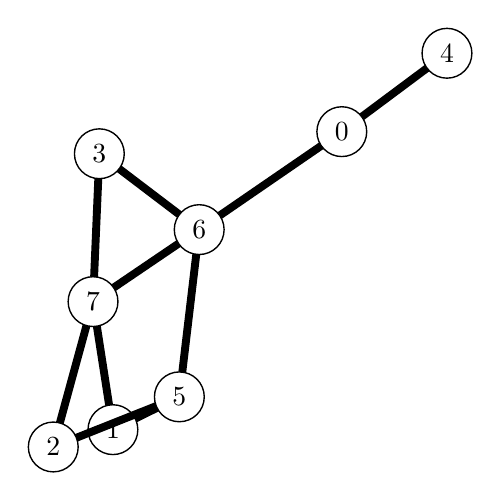
\begin{tikzpicture}
\definecolor{cv0}{rgb}{0.0,0.0,0.0}
\definecolor{cfv0}{rgb}{1.0,1.0,1.0}
\definecolor{clv0}{rgb}{0.0,0.0,0.0}
\definecolor{cv1}{rgb}{0.0,0.0,0.0}
\definecolor{cfv1}{rgb}{1.0,1.0,1.0}
\definecolor{clv1}{rgb}{0.0,0.0,0.0}
\definecolor{cv2}{rgb}{0.0,0.0,0.0}
\definecolor{cfv2}{rgb}{1.0,1.0,1.0}
\definecolor{clv2}{rgb}{0.0,0.0,0.0}
\definecolor{cv3}{rgb}{0.0,0.0,0.0}
\definecolor{cfv3}{rgb}{1.0,1.0,1.0}
\definecolor{clv3}{rgb}{0.0,0.0,0.0}
\definecolor{cv4}{rgb}{0.0,0.0,0.0}
\definecolor{cfv4}{rgb}{1.0,1.0,1.0}
\definecolor{clv4}{rgb}{0.0,0.0,0.0}
\definecolor{cv5}{rgb}{0.0,0.0,0.0}
\definecolor{cfv5}{rgb}{1.0,1.0,1.0}
\definecolor{clv5}{rgb}{0.0,0.0,0.0}
\definecolor{cv6}{rgb}{0.0,0.0,0.0}
\definecolor{cfv6}{rgb}{1.0,1.0,1.0}
\definecolor{clv6}{rgb}{0.0,0.0,0.0}
\definecolor{cv7}{rgb}{0.0,0.0,0.0}
\definecolor{cfv7}{rgb}{1.0,1.0,1.0}
\definecolor{clv7}{rgb}{0.0,0.0,0.0}
\definecolor{cv0v4}{rgb}{0.0,0.0,0.0}
\definecolor{cv0v6}{rgb}{0.0,0.0,0.0}
\definecolor{cv1v5}{rgb}{0.0,0.0,0.0}
\definecolor{cv1v7}{rgb}{0.0,0.0,0.0}
\definecolor{cv2v5}{rgb}{0.0,0.0,0.0}
\definecolor{cv2v7}{rgb}{0.0,0.0,0.0}
\definecolor{cv3v6}{rgb}{0.0,0.0,0.0}
\definecolor{cv3v7}{rgb}{0.0,0.0,0.0}
\definecolor{cv5v6}{rgb}{0.0,0.0,0.0}
\definecolor{cv6v7}{rgb}{0.0,0.0,0.0}
%
\Vertex[style={minimum size=1.0cm,draw=cv0,fill=cfv0,text=clv0,shape=circle},LabelOut=false,L=\hbox{$0$},x=3.6644cm,y=4.0045cm]{v0}
\Vertex[style={minimum size=1.0cm,draw=cv1,fill=cfv1,text=clv1,shape=circle},LabelOut=false,L=\hbox{$1$},x=0.7576cm,y=0.2199cm]{v1}
\Vertex[style={minimum size=1.0cm,draw=cv2,fill=cfv2,text=clv2,shape=circle},LabelOut=false,L=\hbox{$2$},x=0.0cm,y=0.0cm]{v2}
\Vertex[style={minimum size=1.0cm,draw=cv3,fill=cfv3,text=clv3,shape=circle},LabelOut=false,L=\hbox{$3$},x=0.5853cm,y=3.7239cm]{v3}
\Vertex[style={minimum size=1.0cm,draw=cv4,fill=cfv4,text=clv4,shape=circle},LabelOut=false,L=\hbox{$4$},x=5.0cm,y=5.0cm]{v4}
\Vertex[style={minimum size=1.0cm,draw=cv5,fill=cfv5,text=clv5,shape=circle},LabelOut=false,L=\hbox{$5$},x=1.6012cm,y=0.6367cm]{v5}
\Vertex[style={minimum size=1.0cm,draw=cv6,fill=cfv6,text=clv6,shape=circle},LabelOut=false,L=\hbox{$6$},x=1.8533cm,y=2.7604cm]{v6}
\Vertex[style={minimum size=1.0cm,draw=cv7,fill=cfv7,text=clv7,shape=circle},LabelOut=false,L=\hbox{$7$},x=0.5051cm,y=1.846cm]{v7}
%
\Edge[lw=0.1cm,style={color=cv0v4,},](v0)(v4)
\Edge[lw=0.1cm,style={color=cv0v6,},](v0)(v6)
\Edge[lw=0.1cm,style={color=cv1v5,},](v1)(v5)
\Edge[lw=0.1cm,style={color=cv1v7,},](v1)(v7)
\Edge[lw=0.1cm,style={color=cv2v5,},](v2)(v5)
\Edge[lw=0.1cm,style={color=cv2v7,},](v2)(v7)
\Edge[lw=0.1cm,style={color=cv3v6,},](v3)(v6)
\Edge[lw=0.1cm,style={color=cv3v7,},](v3)(v7)
\Edge[lw=0.1cm,style={color=cv5v6,},](v5)(v6)
\Edge[lw=0.1cm,style={color=cv6v7,},](v6)(v7)
%
\end{tikzpicture}
\caption{$dim(G) = 2, edim(G) = 3, mdim(G) = 5$}
\end{figure}


% 10_94590_graph_d2_e3
\begin{figure}[H]
\centering
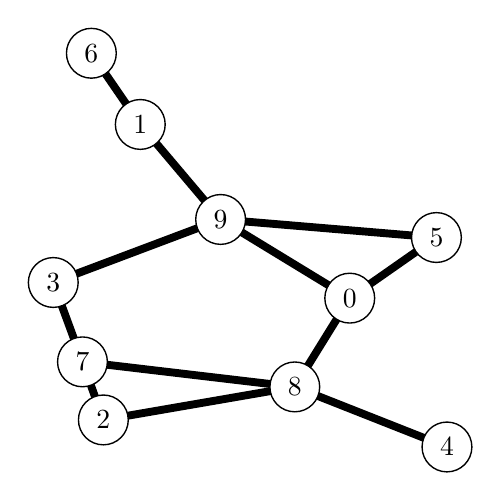
\begin{tikzpicture}
\definecolor{cv0}{rgb}{0.0,0.0,0.0}
\definecolor{cfv0}{rgb}{1.0,1.0,1.0}
\definecolor{clv0}{rgb}{0.0,0.0,0.0}
\definecolor{cv1}{rgb}{0.0,0.0,0.0}
\definecolor{cfv1}{rgb}{1.0,1.0,1.0}
\definecolor{clv1}{rgb}{0.0,0.0,0.0}
\definecolor{cv2}{rgb}{0.0,0.0,0.0}
\definecolor{cfv2}{rgb}{1.0,1.0,1.0}
\definecolor{clv2}{rgb}{0.0,0.0,0.0}
\definecolor{cv3}{rgb}{0.0,0.0,0.0}
\definecolor{cfv3}{rgb}{1.0,1.0,1.0}
\definecolor{clv3}{rgb}{0.0,0.0,0.0}
\definecolor{cv4}{rgb}{0.0,0.0,0.0}
\definecolor{cfv4}{rgb}{1.0,1.0,1.0}
\definecolor{clv4}{rgb}{0.0,0.0,0.0}
\definecolor{cv5}{rgb}{0.0,0.0,0.0}
\definecolor{cfv5}{rgb}{1.0,1.0,1.0}
\definecolor{clv5}{rgb}{0.0,0.0,0.0}
\definecolor{cv6}{rgb}{0.0,0.0,0.0}
\definecolor{cfv6}{rgb}{1.0,1.0,1.0}
\definecolor{clv6}{rgb}{0.0,0.0,0.0}
\definecolor{cv7}{rgb}{0.0,0.0,0.0}
\definecolor{cfv7}{rgb}{1.0,1.0,1.0}
\definecolor{clv7}{rgb}{0.0,0.0,0.0}
\definecolor{cv8}{rgb}{0.0,0.0,0.0}
\definecolor{cfv8}{rgb}{1.0,1.0,1.0}
\definecolor{clv8}{rgb}{0.0,0.0,0.0}
\definecolor{cv9}{rgb}{0.0,0.0,0.0}
\definecolor{cfv9}{rgb}{1.0,1.0,1.0}
\definecolor{clv9}{rgb}{0.0,0.0,0.0}
\definecolor{cv0v5}{rgb}{0.0,0.0,0.0}
\definecolor{cv0v8}{rgb}{0.0,0.0,0.0}
\definecolor{cv0v9}{rgb}{0.0,0.0,0.0}
\definecolor{cv1v6}{rgb}{0.0,0.0,0.0}
\definecolor{cv1v9}{rgb}{0.0,0.0,0.0}
\definecolor{cv2v7}{rgb}{0.0,0.0,0.0}
\definecolor{cv2v8}{rgb}{0.0,0.0,0.0}
\definecolor{cv3v7}{rgb}{0.0,0.0,0.0}
\definecolor{cv3v9}{rgb}{0.0,0.0,0.0}
\definecolor{cv4v8}{rgb}{0.0,0.0,0.0}
\definecolor{cv5v9}{rgb}{0.0,0.0,0.0}
\definecolor{cv7v8}{rgb}{0.0,0.0,0.0}
%
\Vertex[style={minimum size=1.0cm,draw=cv0,fill=cfv0,text=clv0,shape=circle},LabelOut=false,L=\hbox{$0$},x=3.7651cm,y=1.8901cm]{v0}
\Vertex[style={minimum size=1.0cm,draw=cv1,fill=cfv1,text=clv1,shape=circle},LabelOut=false,L=\hbox{$1$},x=1.1051cm,y=4.096cm]{v1}
\Vertex[style={minimum size=1.0cm,draw=cv2,fill=cfv2,text=clv2,shape=circle},LabelOut=false,L=\hbox{$2$},x=0.6361cm,y=0.3434cm]{v2}
\Vertex[style={minimum size=1.0cm,draw=cv3,fill=cfv3,text=clv3,shape=circle},LabelOut=false,L=\hbox{$3$},x=0.0cm,y=2.0889cm]{v3}
\Vertex[style={minimum size=1.0cm,draw=cv4,fill=cfv4,text=clv4,shape=circle},LabelOut=false,L=\hbox{$4$},x=5.0cm,y=0.0cm]{v4}
\Vertex[style={minimum size=1.0cm,draw=cv5,fill=cfv5,text=clv5,shape=circle},LabelOut=false,L=\hbox{$5$},x=4.8661cm,y=2.66cm]{v5}
\Vertex[style={minimum size=1.0cm,draw=cv6,fill=cfv6,text=clv6,shape=circle},LabelOut=false,L=\hbox{$6$},x=0.4838cm,y=5.0cm]{v6}
\Vertex[style={minimum size=1.0cm,draw=cv7,fill=cfv7,text=clv7,shape=circle},LabelOut=false,L=\hbox{$7$},x=0.3708cm,y=1.081cm]{v7}
\Vertex[style={minimum size=1.0cm,draw=cv8,fill=cfv8,text=clv8,shape=circle},LabelOut=false,L=\hbox{$8$},x=3.0673cm,y=0.7629cm]{v8}
\Vertex[style={minimum size=1.0cm,draw=cv9,fill=cfv9,text=clv9,shape=circle},LabelOut=false,L=\hbox{$9$},x=2.1254cm,y=2.8894cm]{v9}
%
\Edge[lw=0.1cm,style={color=cv0v5,},](v0)(v5)
\Edge[lw=0.1cm,style={color=cv0v8,},](v0)(v8)
\Edge[lw=0.1cm,style={color=cv0v9,},](v0)(v9)
\Edge[lw=0.1cm,style={color=cv1v6,},](v1)(v6)
\Edge[lw=0.1cm,style={color=cv1v9,},](v1)(v9)
\Edge[lw=0.1cm,style={color=cv2v7,},](v2)(v7)
\Edge[lw=0.1cm,style={color=cv2v8,},](v2)(v8)
\Edge[lw=0.1cm,style={color=cv3v7,},](v3)(v7)
\Edge[lw=0.1cm,style={color=cv3v9,},](v3)(v9)
\Edge[lw=0.1cm,style={color=cv4v8,},](v4)(v8)
\Edge[lw=0.1cm,style={color=cv5v9,},](v5)(v9)
\Edge[lw=0.1cm,style={color=cv7v8,},](v7)(v8)
%
\end{tikzpicture}
\caption{$dim(G) = 2, edim(G) = 3, mdim(G) = 5$}
\end{figure}


\begin{figure}[H]
    \centering
    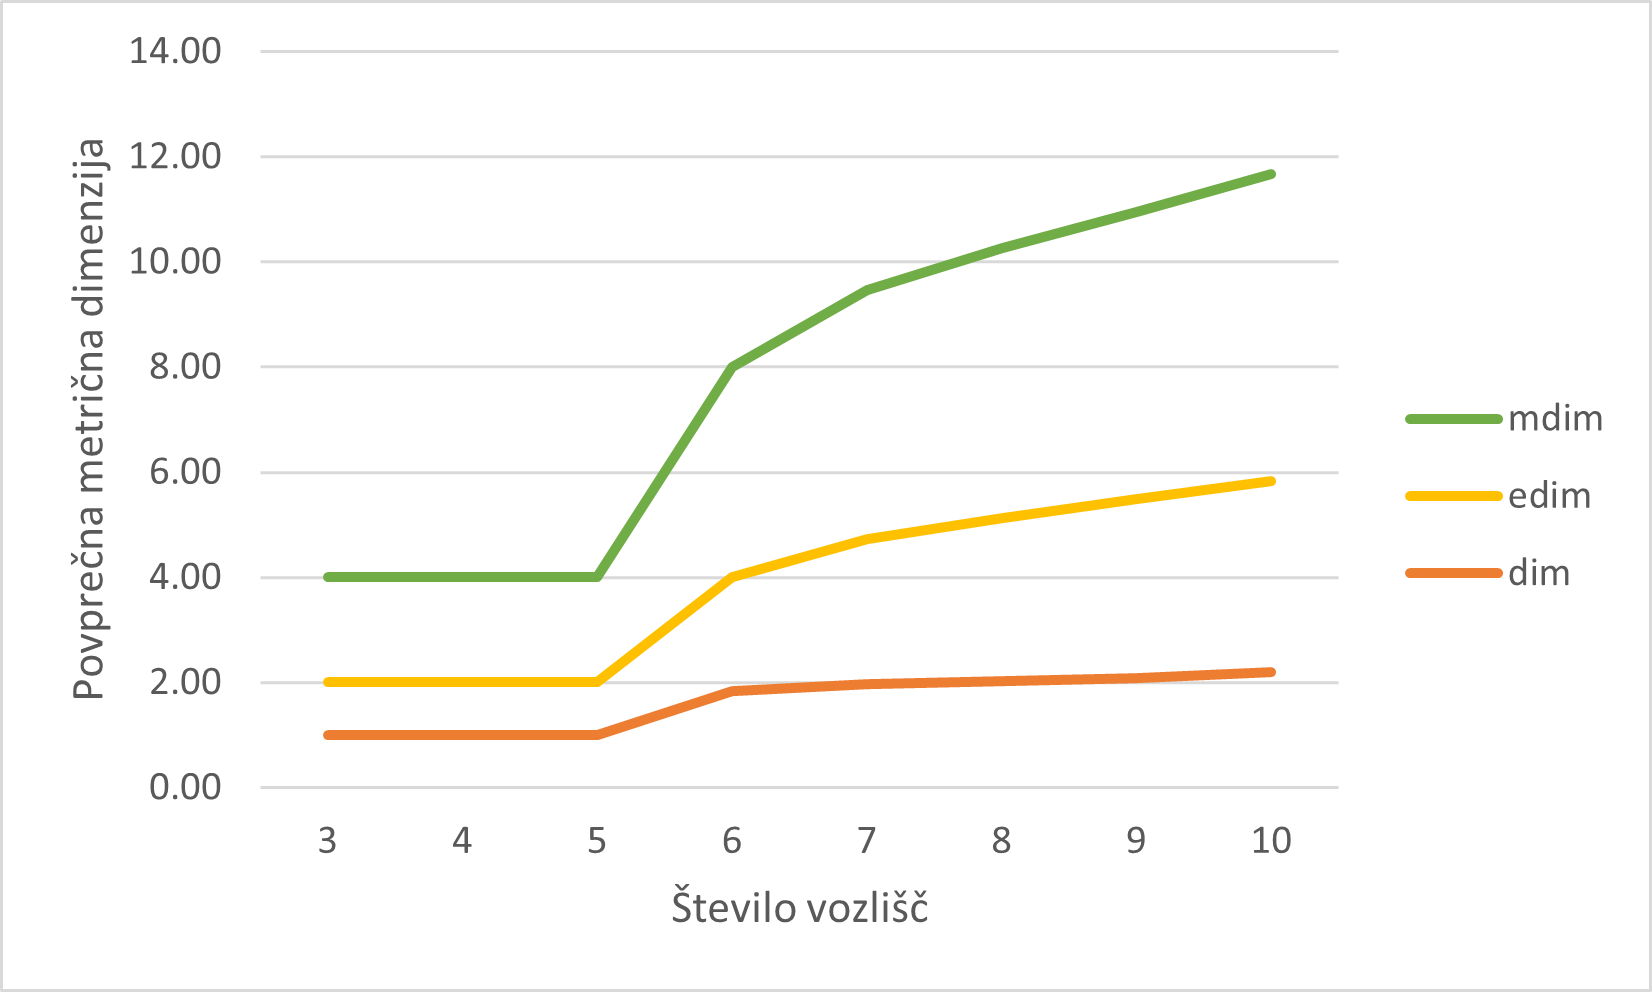
\includegraphics[width=0.7\textwidth]{st_vozl_mean.png}
    \caption{Povprečne metrične dimenzije pri vozliščih}
\end{figure}

\begin{figure}[H]
    \centering
    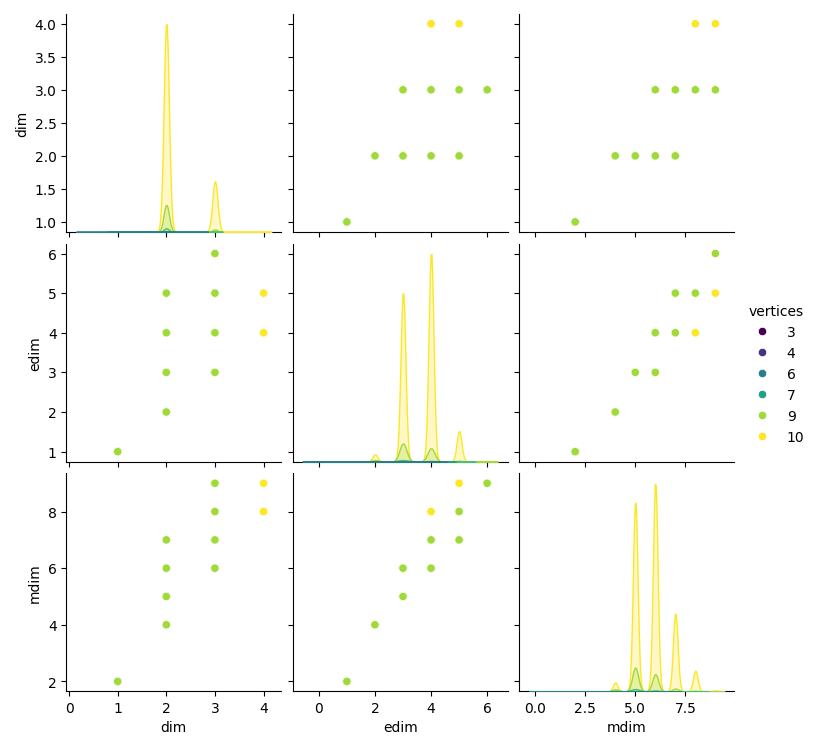
\includegraphics[width=0.9\textwidth]{mdim_pairgraph.png}
    \caption{Korelacija metričnih dimenzij glede na število vozlišč}
\end{figure}



\end{document}
